\documentclass[fleqn]{jbook}
\usepackage{physpub}

\begin{document}

\begin{question}{専攻 問題5}{}

結晶中の各原子(単位体積あたりの個数を $n$ とする)に1個ずつ
電子が存在し、隣り合った原子の間で電子が弱く相互作用している系がある。
ある温度 $T=T_t$ で、この系は1次相転移を示し、
$T \ge T_t$の相(高温相)では、各原子に1個ずつ捕らえられた相互作用の
ない電子からなる系と同じ比熱と帯磁率を示した。
$T \le T_t$の相(低温相)では、弱い原子間の相互作用が摂動となり電子が
ある小さな確率で原子間をとび移るために、比熱、帯磁率は縮退した自由
電子ガスと同じ温度依存性を示した。
しかし、その比熱の絶対値は、自由電子ガスの比熱の表式において、
自由電子の質量 $m_e$ をより大きな値 $m^{\ast}$ (有効質量と呼ぶ)に置き
換えたもので表された。十分低温のため、格子比熱、各相での熱膨張は
無視できるものとして、次の問に答えよ。

\begin{subquestions}
\SubQuestion
  高温相の単位体積あたりの帯磁率、磁場中での比熱を求めよ。
  磁場 $\vec{H}$ と電子との相互作用ハミルトニアンは、
%
  \begin{equation}
    {\cal H} = \sum_i 2\muB \vec{H} \cdot \vec{S_i} \eqname{Q1}
  \end{equation}
%
  で与えられるとする。ここで、$\muB \equiv e \hbar/2m_ec$ は電子の
  ボーア磁子、$\vec{S_i}$ は電子 $i$ のスピン演算子を表す。

\SubQuestion
  低温相の単位体積あたりの比熱は、温度 $T$ の最低次までで、
%
  \begin{equation}
    c\ssub{P} =%
      \frac{\kB^2m^{\ast}}{3\hbar^2}%
      \Bigr(\frac{3n}{8\pi}\Bigr)^{\frac{1}{3}}T  \eqname{Q2}
  \end{equation}
%
  と与えられた($\kB$ : ボルツマン定数)。式 \eqhref{Q2} が温度に
  比例する理由を、有限温度のフェルミ分布関数を用いて定性的に説明せよ。

\vspace*{2mm}
  \hspace*{-2zw}以下の設問では、磁場はかかっていないとし、
  前問で求めた両相の諸量の表式は転移点$T_t$ まで使えるものとする。

\SubQuestion
  上記の1次転移が起こるには、エントロピーの考察から、有効質量
  $m^{\ast}$ と相転移温度 $T_t$ がどのような条件を満たさなければ
  ならないか?

\SubQuestion
  いま、この電子系に圧力 $P$ をかけたところ、相転移温度 $T_t$ が
  上昇し、低温相の比熱より求まる有効質量 $m^{\ast}$ が減少した
  (図参照)。有効質量および相転移温度の圧力依存性は、
  $m_0^{\ast}$ 、 $T_{t0}$ を $P=0$ での有効質量、転移温度として、
%
  \begin{eqnarray}
    m^{\ast} &=& m_0^{\ast} ( 1+aP)^{-1}  \eqname{Q3}\\
    T_t &=& T_{t0} ( 1+bP)  \eqname{Q4}
  \end{eqnarray}
%
  $(a>0,b>0)$ の実験式で与えられた。ある圧力 $P = P_c$ (臨界圧力)
  以上で1次転移が消失するのは、$a$ 、 $b$がどのような条件を満たす
  場合か?

\SubQuestion
  $P_c$、および転移の消失する温度 $T = T_c$ (臨界温度)を、
  $a$ 、$b$ 、$m_0^{\ast}$、$T_{t0}$を用いて表わせ。

\end{subquestions}

  \begin{center}
    \mbox{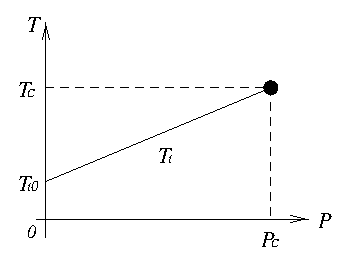
\includegraphics[clip]{1996phy5-1.eps}}
  \end{center}

\end{question}
\begin{answer}{専攻 問題5}{}
\def\sech{\mathop{\rm sech}\nolimits}

\begin{subanswers}
\SubAnswer
  磁場の向きに$z$軸を取り、磁場の強さを $H$ とすると、
  $\vec{H} \cdot \vec{S_i} = H S_{\rm iz}$ となる。
  単位体積あたりの$n$個のスピンの分配関数 $Z$は
%
  \begin{eqnarray*}
    Z &=& \sum_{S_{\rm iz}} \exp{(-\beta {\cal H})}%
       =  \sum_{S_{\rm iz}} \exp{(-\sum_{i}2\muB H S_{\rm iz} \beta)}%
       =  \sum_{S_{\rm iz}} \prod_{i} \exp{(-2\muB H S_{\rm iz} \beta)}\\
      &=& \prod_{i=1}^{n} \sum_{S_{\rm iz}=\pm 1/2}\bquad \exp{(-2\muB H S_{\rm iz} \beta)}%
       =  \bigl[ 2\cosh{(\muB H \beta)} \bigr]^n
  \end{eqnarray*}
%
  となる。自由エネルギー $F$ と内部エネルギー$U$ は
%
  \begin{eqnarray*}
    F &=& -\frac{1}{\beta} \log Z%
       =  -\frac{1}{\beta} n\log{[2\cosh{(\muB H \beta)}]}\\
    U &=& -\Partial{}{\beta} \log Z%
       =  -n \muB H \tanh{(\muB H \beta)}
  \end{eqnarray*}
%
  よって磁化$M$、帯磁率$\chi$、比熱$C$は、
%
  \begin{eqnarray*}
    M &=& - \Partial{F}{H}%
       =  n \muB\tanh{(\muB H \beta)} \\
 \chi\,\, &=& \lim_{H\to 0} \Partial{M}{H}%
       =  \lim_{H\to 0} n \muB^2 \beta \sech^2{(\muB H \beta)}%
       =  n \muB^2 \beta\\
    C &=& \Partial{U}{T}%
       = -\kB \beta^2 \Partial{}{\beta} U%
       = n \kB  \muB^2 \beta^2 H^2 \sech^2{(\muB H \beta)}
  \end{eqnarray*}
%
  となる。

\SubAnswer
  \parbox[t]{105mm}{
  低温相においては、$n$個の電子のうち、$\kB T/\epsilon_F$程度の割合の
  電子が、およそ$\kB T$程度のエネルギーの幅の中にある。従って、
  内部エネルギーの$T=0$の時との差を$\IDelta U$とすると、
%
  \[ \IDelta U \sim n \frac{\kB T}{\epsilon_F}\times \kB T \hspace{15mm}%
     \Yueni%
     C = \Partial{\IDelta U}{T} \propto T \]
%
  となる。
  }\parbox[t]{55mm}{\vspace*{-30mm}
  \begin{center}
    \mbox{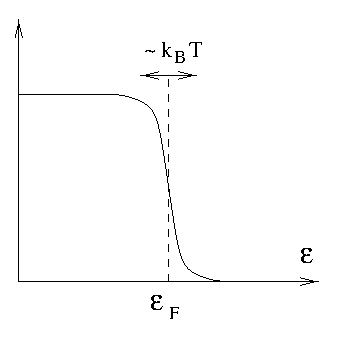
\includegraphics[clip]{1996phy5-2.eps}}
  \end{center}}

\SubAnswer
  1次相転移では、転移点 $T\!=\!T_t$において、低温相の自由エネルギー
  $F_{\rm L}$と高温相のそれ $F_{\rm H}$は一致し、その一階微分は
  一致しない。$T\!>\!T_t$で高温相となるためには、高温相の方が自由
  エネルギーが低くなくてはならない。すなわち、
%
  \[ F_{\rm L}|_{T=T_t} = F_{\rm H}|_{T=T_t} \hspace{15mm}%
    \Partial{F_{\rm L}}{T}\Bigm|_{T=T_t} > \Partial{F_{\rm H}}{T}\Bigm|_{T=T_t}\]
%
  ところでエントロピー $S$ は $S\!=\!-\tPartial{F}{T}$で
  与えられるので、これより、
%
  \[ S_{\rm L}|_{T=T_t} < S_{\rm H}|_{T=T_t} \]
%
  であることがわかる。これが1次相転移が起こるための条件である。
  具体的にこの量を計算する。

  高温相では、磁場がかかっていないので、設問{\bf 1.}より
%
  \[ F_{\rm H}|_{T=T_t} = -\frac{n}{\beta}\log{2} \hspace{15mm}%
     S_{\rm H}|_{T=T_t} = n\kB \log{2} \]
%
  低温相では、設問{\bf 2.}で与えられた比熱の表式と定圧比熱の
  定義式から
%
  \[ c\ssub{P}%
     = T \Bigl( \Partial{S_{\rm L}}{T} \Bigr)_p%
     = \frac{\kB^2m^{\ast}}{3\hbar^2}%
       \Bigr(\frac{3n}{8\pi}\Bigr)^{\frac{1}{3}}T \hspace{15mm}%
    \Yueni S_{\rm L}|_{T=T_t} = \frac{\kB^2m^\ast}{3\hbar^2}%
       \Bigl(\frac{3n}{8\pi}\Bigr)^{1/3}T_t \]
%
  よって1次相転移が起こるための条件は
%
  \[ \frac{\kB ^2m^\ast}{3\hbar^2}%
     \Bigl(\frac{3n}{8\pi}\Bigr)^{1/3}T_t < n\kB \log{2} \]
%
  である。

\SubAnswer
  \parbox[t]{90mm}{
  1次相転移が臨界圧力$P\!=\!P_c$で消失するとは、
  $S_{\rm L}|_{T=T_t}\!=\!S_{\rm H}|_{T=T_t}$となることである。
  $P\!<\!P_c$で$S_{\rm L}|_{T=T_t}\!<\!S_{\rm H}|_{T=T_t}$であった
  のが、圧力を上げることで$S_{\rm L}|_{T=T_t}\!=\!S_{\rm H}|_{T=T_t}$
  となるためには、$S_{\rm H}|_{T=T_t}$が定数であることから
  $S_{\rm L}|_{T=T_t}$が圧力に対して右図の様な増加関数でなければ
  ならない。
  $S_{\rm L}|_{T=T_t}$を式\eqhref{Q3},\eqhref{Q4}を用いて表すと、
%
  \[ S_{\rm L}|_{T=T_t} = \frac{\kB ^2m_0^\ast}{3\hbar^2(1+aP)}%
     \Bigl(\frac{3n}{8\pi}\Bigr)^{1/3} T_{t0}(1+bP) \]
%
  これが $P$の増加関数となるためには%
  \[ b > a \]
でなければならず、また
$P\to \infty$で$S_{\rm L}|_{T=T_t}>S_{\rm H}$, すなわち\[
n\kB\log{2}<\frac{\kB ^2m_0^\ast}{3\hbar^2}%
     \Bigl(\frac{3n}{8\pi}\Bigr)^{1/3} T_{t0}\frac{b}{a}
\]
  でなければならない。
  }\parbox[t]{70mm}{
  \begin{center}
    \mbox{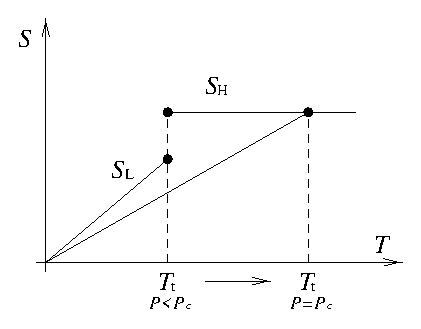
\includegraphics[clip]{1996phy5-3.eps}}
  \end{center}}

\SubAnswer
  $P_c$の満たすべき方程式は前問より次の通り。
%
  \[ \frac{\kB^2m_0^\ast}{3\hbar^2(1+aP_c)}%
     \Bigl(\frac{3n}{8\pi}\Bigr)^{1/3} T_{t0}(1+bP_c)
     = n\kB \log{2} \]
%
  これより、
%
  \[ P_c = \frac{\kappa-1}{b-a\kappa} \hspace{15mm}
     T_c = T_{t0}(1+bP_c)
         = T_{t0} \frac{(b-a)\kappa}{b-a\kappa} \]
  \[ {\rm where}\quad%
     \kappa \equiv \frac{3n\hbar^2\log{2}}{\kB m_0^\ast}%
              \Bigl( \frac{8\pi}{3n} \Bigr)^{1/3}\frac{1}{T_{t0}} \]

\end{subanswers}
\end{answer}


\end{document}
